\chapter{Tecniche di produzione additive}\label{chp:TecnicheAdditive}
Con l'espressione \emph{Tecnologie additive} ci si riferisce all'insieme dei processi di trasformazione volti all'ottenimento del volume e della geometria del componente tramite l'aggiunta progressiva di materiale in assenza di stampi.

\section{Fasi comuni dei processi additivi}

\begin{wrapfloat}{figure}{O}{0pt}
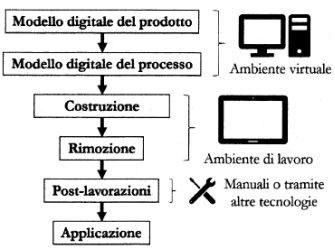
\includegraphics[width = 0.4\textwidth]{ProcAdditivi}
\caption{Operazioni comuni ai processi additivi}
\label{fig:ProcAdditivi}
\end{wrapfloat}

Tutti i processi additivi partono da una rappresentazione virtuale del modello realizzata tramite \ac{CAD}.
La presenza di un modello digitale del prodotto è un prerequisito vincolante.
I processi additivi utilizzano una presentazione del solido detta \ac{STL}.
Le superfici esterne sono rappresentate tramite una discretizzazione (mesh) di elementi triangolari.

Ciascun elemento triangolare (o facet) è caratterizzato dalle nove coordinate cartesiane ($X$, $Y$, $Z$) dei suoi tre vertici ($v_1$, $v_2$, $v_3$) e dalle tre componenti ($i$, $j$, $k$) del versore uscente dalla superficie .

Il passaggio da una rappresentazione B-Rep ad una discretizzazione tramite triangoli comporta un'approssimazione delle superfici matematiche del componente.

La maggior parte degli ambienti \ac{CAD} consente di fissare un parametro detto corda massima, ovvero la massima distanza tra la discretizzazione triangolare e le superfici matematiche.

Negli ultimi anni sono stati proposti nuovi formati con lo scopo di includere ulteriori informazioni riguardo il modello e ridurre la quantità di memoria allocata tramite compressione.

È necessario assicurarsi che l'insieme dei triangoli rappresentati le superfici di un solido reale.
È necessario correggere eventuali zone di criticità nella discretizzazione.
Esistono numerosi software dedicati alla verifica e riparazione di file \ac{STL}.

Dopo le considerazioni circa quale ambiente di sviluppo sia più opportuno.
Si ha la creazione  di una rappresentazione virtuale del lavoro di stampa.
Comprende gli aspetti geometrici, come ad esempio quanti e quali oggetti debbano essere realizzati, la loro posizione e il loro orientamento all'interno dell'area di lavoro.

Il primo passo per la modellazione del processo addittivo è la definizione dell'area di lavoro.
La rappresentazione in ambiente virtuale dell'area di lavoro include, oltre alla geometria dell'area di lavoro, il sistema di riferimento cartesiano della macchina.

Per consentire la lavorazione, il prodotto dovrà essere situato all'interno dell'area di lavoro della macchina.
A livello di rappresentazione digitale, ciò si traduce in una serie di rotazioni e traslazioni del sistema di riferimento locale del modello rispetto al sistema di riferimento della macchina.
L'orientamento e la posizione del componente rispetto al sistema di riferimento macchina hanno un'importanza fondamentale nel determinare le proprietà fisiche e geometriche del prodotto, nonché i tempi e la quantità di materiale necessari e la sua realizzazione.

La scelta della posizione e dell'orientamento di ciascun modello avrà quindi un'incidenza fondamentale nel determinare il numero di componenti realizzabili tramite il medesimo processo produttivo. L'operazione di orientamento e collocamento dei modelli all'interno dell'area di lavoro prende il nome di \emph{nesting}.

Nella quasi totalità delle tecnologie additive la geometria tridimensionale del prodotto è ottenuta tramite la sovrapposizione di strati piani di materiale detti \eng{layers} generati in sequenza.
L'area di lavoro è suddivisa tramite una serie di piani normali a $Z$ pari all'altezza del \eng{layer}.
Con lo \eng{slicing} il modello è rappresentato come sovrapposizione di \eng{layer}.
L'approssimazione introdotta con lo \eng{slicing} migliora al ridursi dello spessore degli strati $h_L$.
L'altezza $h_C$ della generica cuspide dipende non solo dalla altezza $h_L$ del layer, anche dall'orientamento della mesh \ac{STL} ovvero dal vettore normale $\widehat{n}$ 
\begin{equation}
h_C = h_L |\cos(\alpha)| \quad \forall \alpha \in ]0:\pi[ \label{eqn:Slicing}
\end{equation}
I parametri fanno riferimento alla figura \ref{fig:Slicing}.
\begin{figure}
\centering
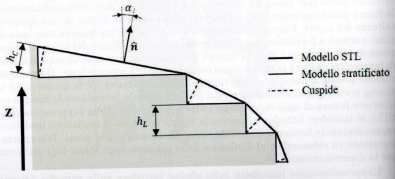
\includegraphics[width = 0.7\textwidth]{Slicing}
\caption{Rappresentazione dei parametri dell'equazione \eqref{eqn:Slicing}}
\label{fig:Slicing}
\end{figure}

Le features piane che richiedono un grado di dettaglio elevato sono, se possibile, realizzare nel piano $XY$.
Quando si devono realizzare due componenti destinati all'accoppiamento è sempre opportuno che le superficie a contatto vengano costruite con il medesimo orientamento rispetto al piano di stampa.
Una volta completato il modello digitale del processo, esso viene convertito da un opportuno software nelle istruzioni macchina necessarie alla sua attuazione.
Tutte le operazioni preparatorie finora descritte siano svolte in ambiente virtuale e non necessitano la prossimità tra operatore e macchina.
Le modalità con cui il materiale viene trasformato per andare  a costruire il componente finale dipendono fortemente dalla tecnologia utilizzata.
L'operatore può controllare l'area di lavoro in maniera diretta o indiretta.
La rimozione del prodotto dall'area di lavoro risulta spesso critica.
Può essere necessario un tempo di attesa tra la fine della costruzione del pezzo e la rimozione del componente.
Molti processi additivi necessitano di introdurre nella zona di lavoro una quantità di materiale di partenza superiore a quella trasformata per formare il pezzo finale.
I pezzi ottenuti da tecnologia additiva, una volta rimossi dalla zona di costruzione, sono spesso inadatti alla messa in opera diretta nella maggior parte delle applicazioni di interesse industriale.

Una volta terminata la fase di costruzione, il prodotto deve essere rimosso dall'area di lavoro
della macchina
Nei processi additivi questa operazione risulta spesso critica e può richiedere particolari
accorgimenti per preservare la qualità del prodotto, dell'ambiente di lavoro e della sicurezza
degli operatori. Questa fase richiede solitamente l'impiego di specifiche attrezzature manuali
o robotizzate
A seconda della tecnologia impiegata, può essere necessario un tempo di attesa tra la fine
della costruzione del pezzo e la rimozione del componente
Nei processi che agiscono per via termica tale tempo di attesa consente un rilassamento
delle tensioni di raffreddamento necessario ad evitare deformazioni incontrollate del
prodotto
Se la costruzione avviene in presenza di gas pericolosi per l'essere umano o per l'ambiente,
essi devono essere aspirati (tramite opportuni sistemi di filtraggio) prima che la zona di
costruzione sia messa in contatto con l'ambiente esterno.

In molti processi il distacco del pezzo dalla macchina richiede l'ausilio di opportune
attrezzature (manuali o robotizzate) che consentano di evitare il danneggiamento del
prodotto e dei componenti della macchina stessa
Un aspetto particolarmente importante legato alla rimozione del componente dalla zona di
lavoro è il recupero del materiale non trasformato eventualmente presente in essa
Infatti, molti processi additivi necessitano di introdurre nella zona di lavoro una quantità di
materiale di partenza superiore a quella trasformata per formare il pezzo finale; il materiale
in eccesso deve dunque essere opportunamente raccolto per poter essere riutilizzato
(totalmente o in percentuali controllate) nelle produzioni successive

I pezzi ottenuti da tecnologia additiva, una volta rimossi dalla zona di costruzione, sono
spesso inadatti alla messa in opera diretta nella maggior parte delle applicazioni di interesse
industriale
Si possono dunque rendere necessarie varie operazioni sulle parti ottenute al fine di
raggiungere le caratteristiche geometriche e fisiche imposte dal progetto
Tali operazioni si configurano quindi come fasi successive all'interno del ciclo produttivo del
componente e possono raggiungere gradi di complessità molto differenti a seconda della
tecnologia impiegata e delle richieste progettuali

Tra le operazioni più comunemente adottate a valle dei processi additivi vi sono:
\begin{description}
\item[Rimozione delle strutture ausiliarie], ovvero di tutte le eventuali porzioni di materiale
trasformato necessarie alla costruzione del pezzo, ma non alla sua messa in opera.
\item[Pulizia del pezzo] con rimozione dell'eventuale materiale non trasformato che residua dopo
l'estrazione del pezzo dall'area di costruzione.
\item[Trattamenti termici] fisici o chimici, necessari a conferire alla parte specifiche proprietà meccaniche o fisiche.
\item[Finitura superficiale] in particolare al fine ridurre l'effetto "a gradini" indotto dalla
stratificazione sulle superfici esterne.
\item[Ulteriori operazioni post-processo] possono includere verniciatura, rivestimento, infiltrazione ed altri.
\end{description}

Le prime applicazioni dei processi additivi si sono avute nel campo dello sviluppo prodotto
per l'ottenimento di prototipi
La flessibilità delle tecnologie additive, infatti, consente di ottenere geometrie tridimensionali
di forma complessa in tempi ristretti rispetto alle tradizionali tecniche di prototipazione
In seguito, le accuratezze dimensionali ottenibili e la ripetibilità del processo hanno
consentito a molte tecnologie di produrre componenti che vadano ad inserirsi all'interno di
assiemi complessi (accoppiandosi agli altri elementi funzionali).

Le proprietà fisiche e meccaniche che possono essere raggiunte tramite alcune tecnologie
additive sono ad oggi comparabili con quelle dei prodotti da "processi tradizionali"
L'applicabilità di una tecnologia additiva in luogo di altri metodi per la produzione di un dato
componente dipende dalle specifiche della tecnologia medesima e del progetto
Tali tecnologie risultano spesso convenienti economicamente rispetto ai metodi
"tradizionali" nel caso di geometrie complesse e piccoli lotti di produzione
Infatti, la costruzione per strati consente il superamento di molti vincoli legati ad altri
processi, consentendo di sostituire un ciclo produttivo in più fasi.
Inoltre, l'assenza di attrezzature fisse legate alla geometria del componente consente di
svincolare il costo unitario del prodotto dalle dimensioni del lotto produttivo.

I vantaggi derivanti dall'impiego di tecnologie additive possono essere colti appieno solo
tramite un'opportuna progettazione che tenga conto di potenzialità e vincoli degli specifici
processi
A tal fine, è fondamentale che i progettisti siano informati riguardo i nuovi strumenti
tecnologici, introdotti sul mercato ad un ritmo sempre più serrato

\section{Classificazione}
Il panorama delle tecnologie additive risulta estremamente variegato ed in continua
evoluzione
Fornire una classificazione soddisfacente di tali processi in grado di porre ordine in questo
scenario risulta complicato
Vedremo una classificazione basata su:
\begin{itemize}
\item Materiale di partenza
\item Strategia di stratificazione
\item Strategia di costruzione del layer
\end{itemize}

Nel seguito ciascuna di queste tre voci sarà brevemente definita, con la presentazione delle
categorie che la compongono e delle relative peculiarità

I materiali di partenza per le tecnologie additive possono essere:
\begin{itemize}
\item Liquidi
\item Viscosi
\item Pulviscolari
\item Solidi
\end{itemize}

\subsection{Materiali liquidi}
I principali materiali allo stato liquido utilizzati nel campo delle tecnologie additive sono le
resine \textbf{fotopolimeriche}, ovvero resine termoindurenti in grado di polimerizzare tramite \textbf{fotopolimerizzazione}.
La fotopolimerizzazione è il meccanismo chimico-fisico tramite il quale alcuni materiali
polimerici modificano le proprie caratteristiche quando colpiti da una radiazione luminosa
Il risultato della fotopolimerizzazione è un polimero termoindurente solido
A seconda del tipo di resina utilizzata, la polimerizzazione può avvenire seguendo due
diversi meccanismi:
\begin{description}
\item[Fotopolimerizzazione radicalica] nella quale la catena polimerica si forma tramite la
successiva addizione di radicali liberi. E' un meccanismo tipico delle resine acriliche.
\item[Fotopolimerizzazione cationica] nella quale i monomeri assorbono una carica che li rende
reattivi, consentendone l'aggregamento ad altri monomeri per la formazione del polimero. É
un meccanismo tipico delle resine epossidiche
\end{description}

In entrambi i casi, è necessaria la presenza all'interno della resina liquida di un particolare
elemento chimico -detto fotoiniziatore- che una volta sottoposto a radiazione luminosa
rilascia le sostanze necessarie ad innescare la polimerizzazione del materiale
La fotopolimerizzazione radicalica risulta più veloce di quella cationica, e questo la rende
particolarmente favorevole per contenere i tempi necessari al processo additivo tramite
fotopolimerizzazione selettiva.
Di contro, le resine epossidiche mostrano una minor contrazione volumetrica durante la
polimerizzazione, con conseguente riduzione delle distorsioni nel pezzo finale
Perciò, queste famiglie di monomeri sono attualmente spesso incluse nella composizione
delle resine commerciali.
La necessità di innescare la fotopolimerizzazione pone un importante limite ai materiali
trasformabili tramite questo meccanismo.
Le resine liquide adottate nel processo di stereolitografia possono contenere altri elementi
in grado di a conferire al componente finale particolari caratteristiche fisiche.

\subsection{Materiali viscosi}
Ricordando che la deformazione dei materiali viscosi è funzione non solo del carico applicato,
ma anche della sua durata.
I materiali reali hanno una, seppur piccola, componente di deformazione elastica, la quale
deve essere tenuta in considerazione durante il processo di trasformazione.
I materiali di interesse per i processi di trasformazione additiva includono polimeri
termoplastici, impasti ceramici, cemento, paste alimentari ed altri.
Tali materiali vengono mantenuti allo stato viscoso durante il processo di costruzione della
geometria tridimensionale.
Una volta modellati, vengono quindi sottoposti a trattamenti finalizzati a conferire al
manufatto le proprietà meccaniche desiderate, in particolare in termini di rigidezza
Tali trattamenti possono consistere in raffreddamenti, cicli di cottura, essiccazione, o altro.

\subsection{Polveri}
I materiali in forma pulviscolare sono costituiti da particelle solide di granulometria
solitamente inferiore ai $100\unit{\um}$.
Tali materiali trovano grande impiego nel campo delle tecnologie additive, grazie alla loro
estrema versatilità ed alla possibilità di mescolare polveri di diversa natura, ottenendo così
particolari proprietà fisico-chimiche del prodotto finito.
Le classi di materiali processate nel campo delle tecnologie additive includono polimeri
termoplastici, metalli e minerali come le ceramiche ed il silice.
Il consolidamento delle polveri per ottenere un solido continuo tramite tecnologie additive
avviene attraverso sinterizzazione e/o fusione.

Si possono distinguere quattro principali meccanismi di unione:
\begin{description}
\item[Sinterizzazione allo stato solido]
\item[Legame chimico]
\item[Sinterizzazione per fusione localizzata]
\item[Rifusione completa]
\end{description}
I processi additivi possono utilizzare uno o più di questi meccanismi per ottenere un solido
a partire dal materiale pulviscolare

La sinterizzazione allo stato solido avviene ponendo dei grani di polvere adiacenti in un
ambiente che ne aumenti l'energia superficiale specifica rispetto alle condizioni ambientali
(questo può essere fatto, ad esempio, aumentando la temperatura o la pressione).
All'aumentare dell'energia superficiale specifica, per minimizzare l'energia superficiale totale
del sistema, le particelle di polvere tenderanno ad unirsi come in \ref{fig:SSSinter} B) , riducendo così la superficie totale. Tale fenomeno avviene a temperature anche inferiori a quella di fusione del materiale, senza quindi nessun passaggio attraverso lo stato liquido.
\begin{figure}
\centering
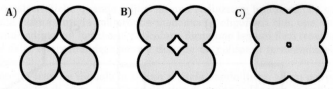
\includegraphics[width = 0.7\textwidth]{SSSinter}
\caption{Particolare sulla sinterizzazione allo stato solido}
\label{fig:SSSinter}
\end{figure}

Il consolidamento per via chimica si basa su reazioni chimiche attivate termicamente (tra
polveri differenti o tra la polvere e altri elementi presenti nell'ambiente di lavoro) che portano
alla generazione di sottoprodotti che fungono da leganti
Si ha quindi un incollaggio delle polveri solide tramite un secondo prodotto. Il risultato di
questo meccanismo di consolidamento è dunque un materiale composito costituito dal
materiale di base e dal legante
La resistenza del componente finale dipende dunque dalle forze adesive tra polvere e
legante, e non dalle caratteristiche proprie del materiale di base
Inoltre, questo meccanismo di consolidamento porta a parti con porosità generalmente
elevate, poiché il legante non riesce a riempire efficacemente i meati tra i grani di polvere

Nella fusione localizzata si verifica il passaggio allo stato liquido di alcune zone della polvere.
Tali zone possono essere dovute ad una composizione eterogenea che favorisce la fusione
del componente bassofondente o ad un apporto di calore sufficiente a rifondere solo la parte
esterna del granello; questa seconda tecnica è più facilmente applicabile nei materiali che
presentano bassa conduttività termica (come ad esempio i polimeri).
La figura mostra un esempio di rifusione localizzata in cui la superficie dei grani solidi (\ref{fig:LocalFusion} A) passa allo stato liquido (\ref{fig:LocalFusion} B) per poi risolidificarsi in un solido continuo (\ref{fig:LocalFusion}C).

\begin{figure}
\centering
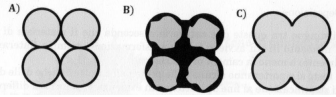
\includegraphics[width = 0.7\textwidth]{LocalFusion}
\caption{Particolare sul funzionamento della fusione localizzata}
\label{fig:LocalFusion}
\end{figure}

Nell'ultimo metodo di consolidamento, la rifusione completa, si assiste al passaggio di tutti i
granelli di materiale allo stato liquido con successiva solidificazione in un solido unico.
La quasi totalità dei processi additivi a letto di polvere utilizza ad oggi la fusione localizzata
o la rifusione completa per la sinterizzazione delle polveri.
Esistono inoltre processi additivi in cui le polveri vengono bagnate da un legante chimico
che funge da collante tra i granelli di solido. Valgono in tal caso le stesse considerazioni
esposte nel caso della sinterizzazione per legame chimico.
Tipicamente questi processi sono seguiti da un trattamento termico durante il quale il
legante viene dissolto e si instaura uno degli altri meccanismi di sinterizzazione per via
termica descritti in precedenza.

\subsection{Materiali Solidi}
I processi additivi che utilizzano materiali di partenza allo stato solido (con forma diversa da
quella pulviscolare) sono attualmente pochi e con limitati campi di applicazione.
Ciò è da imputarsi principalmente alle difficoltà che si incontrano nel modellare il materiale
solido per ottenere la forma dell'oggetto finale.
Per questo motivo, all'interno dei processi additivi, si utilizzano per Io più solidi con
geometrie che ne favoriscano la deformabilità, come filamenti e fogli di piccolo spessore.
Si possono poi adoperare sottoprocessi di taglio per conferire al materiale la forma
desiderata.
I materiali solidi usati sono principalmente polimeri termoplastici e metalli
Il meccanismo di consolidamento può essere l'incollaggio, tramite adesivo o solvente,
oppure la saldatura del materiale.

\section{Strategie di solidificazione}
Il componente realizzato con tecnologia additiva è ottenuto per strati successivi di materiale.
Questi strati possono essere ottenuti per:
\begin{itemize}
\item Trasformazione selettiva (Processi a letto di materiale)
\item Deposizione
\end{itemize}
Si distingue tra queste due categorie a seconda che il materiale di partenza, nel momento
in cui avviene la sua trasformazione, riempia (interamente o parzialmente) o meno la
camera di costruzione.

Nella trasformazione selettiva di materiale la camera di costruzione (o almeno la porzione in cui avviene la trasformazione del materiale) è inizialmente piena del materiale di partenza.
Per questo motivo i processi che utilizzano tale strategia sono anche detti a letto di materiale. Il processo procede quindi trasformando solo la porzione del materiale che corrisponde alla geometria del pezzo.
Una volta completata questa trasformazione, l'intera area di lavoro viene ricoperta di materia prima ed il ciclo si ripete.
Al termine del processo, il pezzo si troverà quindi immerso nel materiale di partenza, dal quale dovrà essere estratto.
Ciò comporta in primo luogo la necessità di una operazione di pulizia del pezzo in seguito alla rimozione dalla camera di costruzione. Non sarà quindi possibile costruire parti cave prive di aperture in quanto il materiale non trasformato rimarrebbe intrappolato all'interno.
La dimensione minima delle aperture necessarie a pulire il pezzo dipenderà dalla sua
geometria, dalle caratteristiche del materiale e dal metodo usato per la pulizia.

Nella deposizione, il materiale viene depositato solo in zone scelte della camera di costruzione, la quale è inizialmente occupata da aria o altri gas.
Il primo layer di materiale sarà depositato sulla piattaforma di costruzione (ovvero il pavimento della camera di costruzione), mentre ciascuno dei layers successivi sarà depositato sul precedente.
Questa strategia di stratificazione offre la possibilità di depositare materiali diversi in maniera controllata. Si ha quindi l'opportunità di progettare e realizzare componenti costituiti da più materiali, cosa che non è in genere possibile fare nei processi a letto di materiale.

\section{Strutture di supporto}
A questo punto è opportuno introdurre un tema fondamentale della progettazione per
tecnologie additive, ovvero le strutture di supporto.
Nei processi di deposizione, al fine di avere ad ogni layer una continuità del materiale con la piattaforma di costruzione, il modello non deve presentare zone a sbalzo nella direzione $Z$.

In altri termini, ad ogni strato $i>0$ ciascuna zona trasformata deve trovare sotto di sé del materiale: infatti, se così non fosse, il materiale non potrebbe aderire al resto del componente, ma cadrebbe sulla piattaforma per effetto della gravità.
Questa considerazione è valida anche per i processi a letto di materiale in cui la materia prima è costituita da un liquido o comunque presenta una densità minore a quella del materiale trasformato.

La figura \ref{fig:MinLoc} mostra un esempio di modello che presenta minimi locali rispetto all'asse Z, mettendo in evidenza come tali zone siano sconnesse dal resto del modello al layer i-esimo.
La presenza di minimi locali può essere in alcuni casi evitata agendo sull'orientamento rispetto all'asse Z del componente in fase di progettazione del processo.
\begin{figure}
\centering
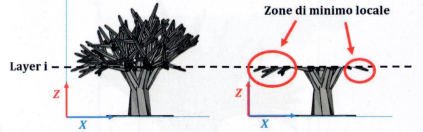
\includegraphics[width = 0.7\textwidth]{MinLoc}
\caption{Minimi locali in un modello 3D sull'asse $Z$}
\label{fig:MinLoc}
\end{figure}

Molto spesso è necessario trasformare zone ausiliarie di materiale, dette supporti, che hanno la funzione di sostenere il materiale trasformato nelle zone a sbalzo del modello. 
La figura \ref{fig:Supporti} mostra in colore blu i supporti aggiunti per sostenere le zone critiche evidenziate nella figura \ref{fig:MinLoc} precedente.

\begin{figure}
\centering
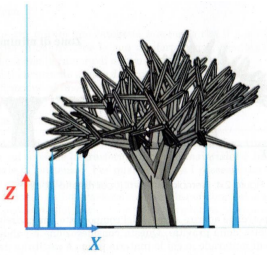
\includegraphics[width = 0.7\textwidth]{Supporti}
\caption{Realizzazione di supporti per i minimi}
\label{fig:Supporti}
\end{figure}

Al termine del processo , il pezzo presenterà dunque delle zone trasformate (le strutture di supporto) che non fanno parte del modello iniziale, ma sono necessarie alla sua realizzazione. Tali strutture dovranno dunque essere rimosse nella fase di post-processo, prima della messa in opera del componente.
I supporti devono essere aggiunti al modello in ambiente virtuale durante la progettazione del processo: esistono a tale scopo numerosi software dedicati.
A seconda delle caratteristiche specifiche della tecnologia e del processo, è possibile utilizzare strutture di supporto di geometrie e dimensioni diverse.

Gli obiettivi che ci si pone durante la progettazione di tali strutture sono:
\begin{itemize}
\item Sostenere efficacemente il materiale in costruzione.
\item Sostenere efficacemente il materiale in costruzione.
\item Ridurre il volume delle strutture di supporto.
\item Facilitare la rimozione dei supporti in post-processo.
\end{itemize}

Al fine di facilitarne la rimozione, i supporti vengono solitamente progettati con sezioni assottigliate in prossimità della parte che fungono da zone di rottura preferenziale (si veda l'esempio di figura \ref{fig:Supporti},in cui i supporti hanno forma conica con sezione minima nel punto di contatto con il pezzo).
Per consentire la rimozione, è inoltre necessario che i supporti siano posizionati in zone raggiungibili dall'operatore e dagli eventuali utensili utilizzati per la loro rimozione.

Oltre che ad evitare la presenza di minimi locali, le strutture di supporto possono essere necessarie anche ad evitare che il materiale appena trasformato si deformi per effetto del proprio peso.

La tendenza del layer a deformarsi sotto l'effetto del peso proprio dipende dalle caratteristiche del materiale, dall'inclinazione rispetto a $Z$ delle superfici e da numerosi parametri di processo come, ad esempio, l'altezza del layer.
Per una certa combinazione di materiale e parametri, è dunque possibile definire un angolo
$\alpha_{lim}$ detto angolo limite rispetto all'asse Z, oltre il quale il materiale non è in grado di sostenere il proprio peso.

\begin{figure}
\centering
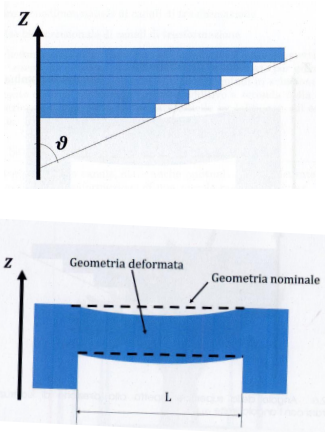
\includegraphics[width = 0.5\textwidth]{Theta_AlphaLim}
\caption{Confronto con l'angolo $\theta$ e l'effetto del peso del materiale su se stesso}
\label{fig:Theta_AlphaLim}
\end{figure}

La figura \ref{fig:Theta_AlphaLim} mostra una rappresentazione dell'angolo $\theta$ da confrontarsi con l'angolo limite $\alpha_{lim}$: si noti come ciascun layer in figura presenti una sezione a sbalzo rispetto allo strato precedente, la cui lunghezza aumenta al crescere di $\theta$.

Una volta noto l'angolo limite, è possibile individuare le superfici che necessitano di supporti, andando a verificare il loro orientamento rispetto alla direzione di costruzione.
La deformazione del materiale sotto l'effetto del peso proprio interessa anche le strutture cosiddette "a ponte", ovvero tutte quelle geometrie sostenute solo agli estremi dal materiale
sottostante.
La figura \ref{fig:Theta_AlphaLim} mostra un esempio di struttura "a ponte" deformata sotto l'effetto del peso proprio.

La deformazione di una struttura a ponte dipende dalla lunghezza della zona sospesa, nonché dalle dimensioni della sezione trasversale.
Si definisce un rapporto massimo tra queste grandezze, oltre il quale sarà necessario ricorrere a strutture di supporto.
Ragionamenti analoghi possono essere condotti nel caso di geometrie a sbalzo. Anche in questo caso si avrà quindi un rapporto massimo tra la sezione della struttura a sbalzo e la sua lunghezza, oltre il quale è necessario fare ricorso a strutture di supporto.
Si sottolinea come la lunghezza limite degli sbalzi sia in genere inferiore, a parità di sezione, a quella delle strutture a ponte.
In alcune tecnologie la progettazione di alcuni di questi elementi, se non supportati, non è ammissibile indipendentemente dalle loro dimensioni.

\section{Strategie per la costruzione dei layer}
A prescindere dalla strategia di trasformazione e dalla tecnica utilizzata per il consolidamento del materiale, è possibile distinguere tre approcci differenti attraverso i quali le tecnologie additive trasformano il materiale di ciascun layer, ovvero:
\begin{description}
\item[Singolo canale di trasformazione]
\item[Vettore monodimensionale di canali di trasformazione]
\item[Matrice bidimensionale di canali di trasformazione]
\end{description}

\subsection{Singolo canale}
Nella strategia a singolo canale, detta anche puntuale, ad ogni istante della lavorazione avviene la trasformazione di una piccola regione del layer.
L'utensile usato per tale trasformazione (sia esso materiale o energetico) viene dunque idealmente considerato come un singolo punto in movimento durante la definizione dei percorsi.
L'utensile può essere attivo o inattivo a seconda che operi o meno la trasformazione del materiale di base.
L'area della porzione di materiale trasformata ad ogni istante dal canale di trasformazione determinerà lo spessore della traccia di materiale trasformata e dunque la definizione ottenibile sul piano del layer.

Ad ogni layer, il canale di trasformazione dovrà ricoprire tutte le aree delle figure piane definite durante la fase di \eng{slicing}.
Per fare ciò, normalmente si distinguono due fasi distinte per ciascun layer: dapprima il canale compie un percorso esterno volto a trasformare il perimetro delle figure piane (\eng{contouring}), mentre nella seconda fase procede a trasformare il materiale all'interno di tali figure (\eng{hatching}).
I percorsi compiuti dal canale di trasformazione durante il \eng{contouring} e l'\eng{hatching} sono detti, rispettivamente, di contorno e di riempimento.

Il tempo di costruzione di ciascun layer dipenderà dunque dall'area delle figure piane in esso contenute.
In particolare, la necessità di effettuare i percorsi di riempimento aumenta il tempo necessario alla costruzione di ciascuno strato in maniera inversamente proporzionale alla velocità del canale di trasformazione e alla porzione di materiale da esso trasformato.
Laddove tali tempi risultino particolarmente onerosi ed i requisiti imposti al componente lo consentano, si preferisce talvolta effettuare un riempimento non completo delle figure piane (e dunque del componente) al fine di ridurre i tempi complessivi del processo.
Per ridurre il tempo di costruzione di ciascuno strato, alcune tecnologie offrono anche la possibilità di adottare più canali di trasformazione (solitamente 2 o 4) che lavorano in parallelo su zone diverse del layer.

\begin{figure}
\centering
\subfloat[][\emph{Esecuzione del contorno del modello}\label{fig:SingCanale1}]
{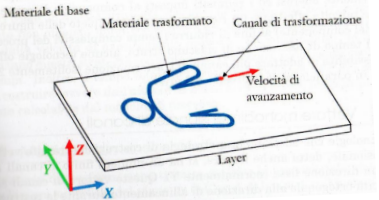
\includegraphics[width = 0.4\textwidth]{SingCanale1}}\quad
\subfloat[][\emph{Riempimento della figura}\label{fig:SingCanale2}]
{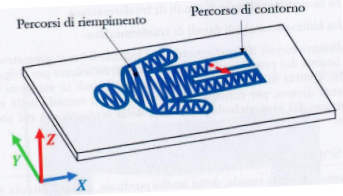
\includegraphics[width = 0.4\textwidth]{SingCanale2}}
\caption{Esecuzione di un modello tramite singolo canale}
\label{fig:SingCanale}
\end{figure}

\subsection{A Vettore}
Nelle tecnologie che adottano una strategia di costruzione tramite vettore monodimensionale di canali, detta anche lineare, si ha un numero finito di canali allineati lungo una direzione fissa (normalmente Y).
Questo vettore di canali si muove con velocità ortogonale alla direzione di allineamento durante la costruzione del layer.
In base alla posizione del vettore, ogni canale si troverà nella condizione attiva o inattiva (cioè trasformerà o meno il materiale di base) a seconda della forma calcolata durante lo \eng{slicing}.
Questa strategia prevede dunque un coordinamento tra l'avanzamento del vettore e l'attuazione acceso/spento di ciascun canale per ottenere la figura comandata; per meglio comprendere, si può pensare all'analogia con la stampa bidimensionale a getto di inchiostro.

La definizione ottenibile nella direzione $Y$ dipenderà dalla porzione di materiale trasformata da ciascun canale e dalla distanza tra canali adiacenti.
La definizione ottenibile nella direzione $X$, invece, dipenderà dalla velocità di avanzamento del vettore di canali.
Si noti come, in questa strategia, il tempo necessario alla costruzione del singolo strato non dipenda dalla geometria delle figure piane contenute nel layer, ma solo dalla velocità di avanzamento imposta.
Di conseguenza, le tecnologie che utilizzano questa strategia consentono di realizzare solidi pieni senza aggravi sui tempi.
Inoltre, il tempo totale del processo dipenderà solo dal numero di layer da costruire (ovvero dall'altezza in z dell'area di lavoro utilizzata) e risulta facilmente calcolabile dal modello di processo.
\begin{figure}
\centering
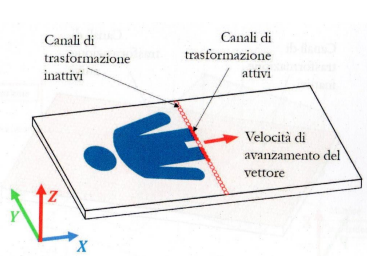
\includegraphics[width = 0.7\textwidth]{Vectorial}
\caption{Modalità di realizzazione a vettore in $Y$}
\label{fig:Vectorial}
\end{figure}

\subsection{Matrice bidimensionale}
Nella strategia di trasformazione tramite matrice bidimensionale di canali, detta anche planare, l'intera superficie del piano $xy$ dell'area di lavoro è suddivisa in piccole regioni, a ciascuna delle quali compete un canale di trasformazione.
L'intera geometria del layer viene dunque trasformata simultaneamente attivando i soli canali corrispondenti alle regioni piene della figura.
Questa strategia prevede dunque una duplice discretizzazione delle geometrie nelle direzioni $X$ ed $Y$, legata alle dimensioni dei canali di trasformazione.
La risoluzione della figura piana è del tutto analoga a quella delle immagini digitali (in questo caso il canale di trasformazione si sostituisce al pixel), tanto che spesso viene espressa in punti per pollice (Dots Per Inch, DPI).

Anche in questo caso, il tempo necessario alla costruzione del singolo strato non è influenzato dalla sua geometria.
Inoltre, qui non si ha nemmeno una dipendenza dalle dimensioni dell'area di lavoro.
Questa strategia, trasformando simultaneamente l'intero layer, consente pertanto solitamente un risparmio considerevole di tempo sull'intero tempo di processo.
\begin{figure}
\centering
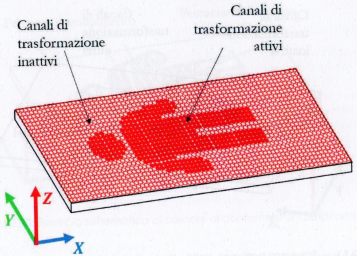
\includegraphics[width = 0.7\textwidth]{Matrix}
\caption{Realizzazione di un modello tramite stampaggio a matrice}
\label{fig:Matrix}
\end{figure}